\chapter{Manual de usuario}
\label{ch:manual_usuario}

\section{Inicio de sesión y registro}

A la hora de abrir la aplicación la primera pantalla que se muestra es la ilustrada en la \fref{man:inicio_sesion}. Esta pantalla consta de un solo botón, pulsarlo desplegará un \emph{pop-up} solicitando una cuenta de Google del dispositivo. Debes seleccionar la cuenta con la que se quiere iniciar la sesión, sea para una nueva cuenta o para una ya existente. Es posible que se solicite la conformidad del usuario para compartir la información de la cuenta con la aplicación, si no se concede esta no podrá funcionar. 

\begin{figure}[H]
    \centering
    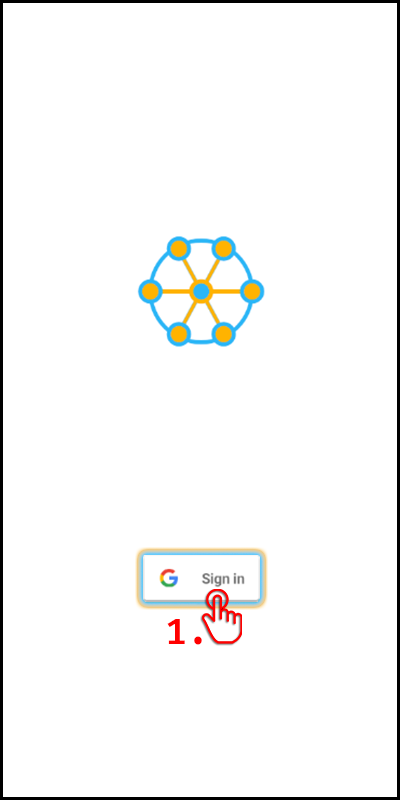
\includegraphics[width=0.25\textwidth]{Manuales/ManualInicioSesion.png}
    \caption{Guía de inicio de sesión.}
    \label{man:inicio_sesion}
\end{figure}

Si la cuenta ya existe, la aplicación te redirigirá a la pantalla principal, desde la cuál se podrán usar las funciones de la aplicación que se pueden consultar en el resto de secciones de este manual. Si la cuenta introducida es nueva en el sistema, la aplicación mostrará una pantalla como la primera que se muestra en la \fref{man:crear_usuario}.

En esta pantalla debes introducir un nombre para identificarte de cara a los usuarios con los que te vincularás. No tiene que ser único en la aplicación ni es necesario que sea tu nombre real, si eres conocido por algún sobrenombre concreto entre la gente con la que compartirás funciones entonces ese apodo será un buena elección. Si entre los usuarios que os vayáis vincular va a haber alguien más que comparta tu mismo nombre, intentad elegir uno que os distinga. Una vez hayas introducido un nombre pulsa en el botón de \textbf{Siguiente} y avanzarás a la pantalla de selección de rol.

En esta aplicación existen dos roles: el de \textbf{Paciente} y el de \textbf{Cuidador}. Todas las funciones giran en torno al paciente. Selecciona aquel rol que represente la clase de papel que tomarás mientras usas la aplicación. Una vez lo hayas hecho vuelve a pulsar en \textbf{Siguiente} para rellenar el resto de datos de tu perfil.

\begin{figure}[H]
    \centering
    \begin{minipage}{0.20\textwidth}
        \centering
        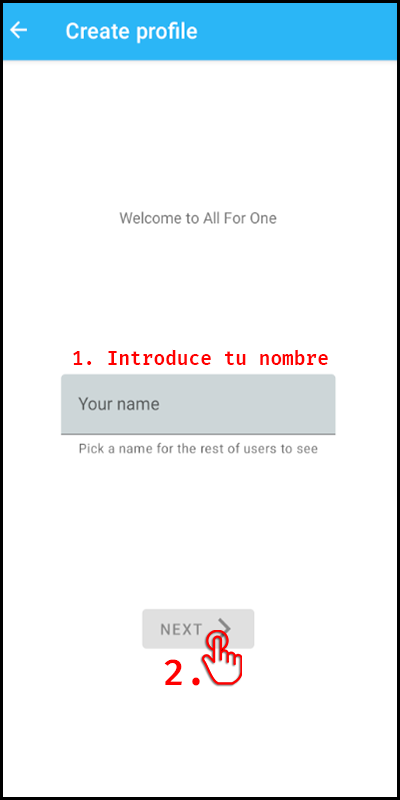
\includegraphics[width=1\textwidth]{Manuales/ManualIntroducirNombre.png}
    \end{minipage}\hfill
    \begin{minipage}{0.20\textwidth}
        \centering
        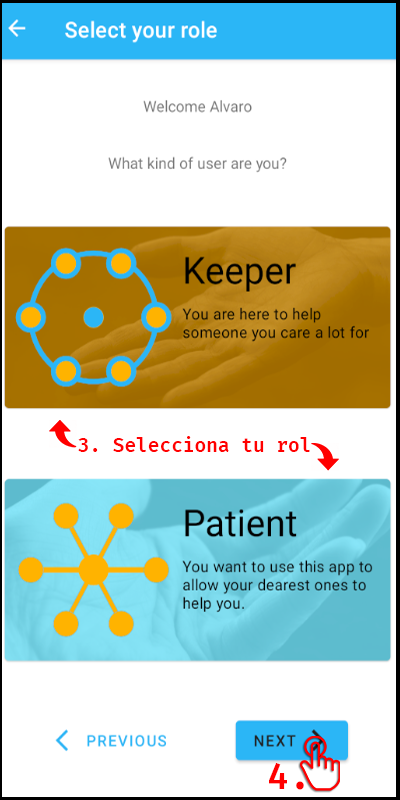
\includegraphics[width=1\textwidth]{Manuales/ManualSeleccionaRol.png}
    \end{minipage}\hfill
    \begin{minipage}{0.20\textwidth}
        \centering
        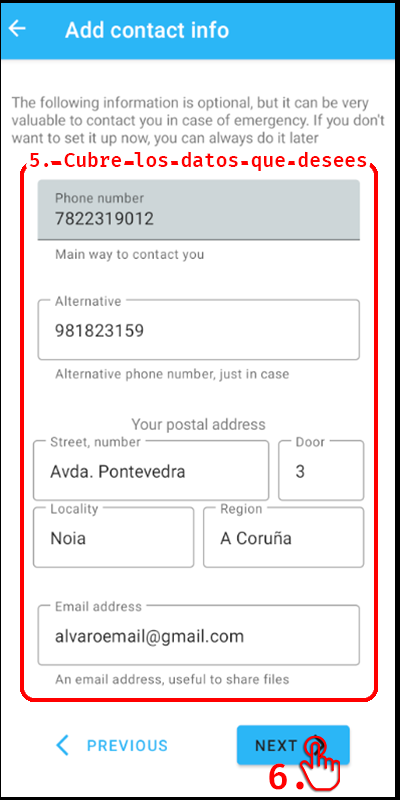
\includegraphics[width=1\textwidth]{Manuales/ManualContacto.png}
    \end{minipage}\hfill
    \begin{minipage}{0.20\textwidth}
        \centering
        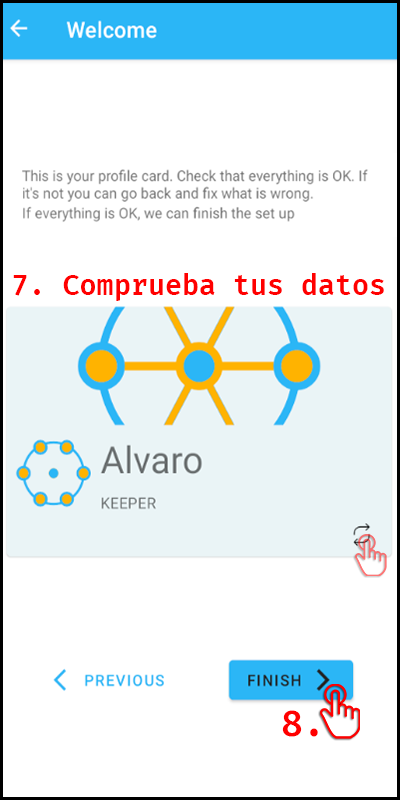
\includegraphics[width=1\textwidth]{Manuales/ManualConfirmacion.png}
    \end{minipage}\hfill
    \caption{Guía de configuración del perfil}
    \label{man:crear_usuario}
\end{figure}

Puedes completar tu perfil con datos adicionales que exponer a los usuarios con los que te vincules para facilitar que se pongan en contacto contigo. Todos estos campos son opcionales, rellenarlos o dejarlos en blanco queda a tu discreción. La lista de datos que puedes rellenar son: \textbf{teléfonos de contacto}, puedes añadir uno principal y uno secundario, por si el principal no está operativo y urge contactar contigo; tu \textbf{tu dirección postal}, para facilitar encuentros en persona si fuese necesario, no tiene que ser tu dirección personal, puede ser la del lugar de trabajo; y \textbf{tu dirección electrónica} o email, de utilidad si algún usuario te quiere enviar algún archivo, por ejemplo. Ten en cuenta que todos estos datos sólo podrán ser vistos por tus usuarios asociados. Cuando hayas acabado avanza con el botón \textbf{Siguiente}.

Finalmente, para terminar la configuración del perfil solamente debes revisar tu información personal en la tarjeta que se te muestra. Por delante se mostrará tu nombre y tu rol, si le das la vuelta con el botón de las flechas podrás ver el resto de tus datos. Si estás conforme con ellos, pulsa en \textbf{Finalizar} para terminar  y avanzar a la aplicación.

\section{Cierre de sesión}

El cierre de sesión es sencillo y similar al de muchas otras aplicaciones. Sólo es necesario acceder a \textbf{Ajustes} y seleccionar la opción de \textbf{Cerrar sesión}.

\section{Vinculación}

Para realizar la vinculación entre dos usuarios el primer requisito es que ambos sean de roles distintos, esto es, uno debe ser Paciente y el otro debe ser Cuidador. Además, el Cuidador no puede estar vinculado y el Paciente debe tener como máximo cinco vínculos activos. Si todo esto se cumple, podréis vincularos.

La vinculación consta de dos pasos: primero el Paciente tendrá que generar un código QR de vinculación y, una vez lo tenga en pantalla, el Cuidador deberá escanearlo. Esto requiere que ambos usuarios estén juntos. Estas dos acciones se explican en detalle a continuación.

\subsection{Paciente - Generar código de vinculación}

El código de vinculación lo generan los pacientes accediendo a la pantalla de \textbf{Vínculos} como se indica en el primer paso de la \fref{man:generar_qr}. Al final de esa pantalla habrá un botón \textbf{Añadir vínculo} que al presionarlo desplegará un código QR válido para escanear y crear el vínculo. Este código es válido durante un minuto.

\begin{figure}[H]
    \centering
    \begin{minipage}{0.30\textwidth}
        \centering
        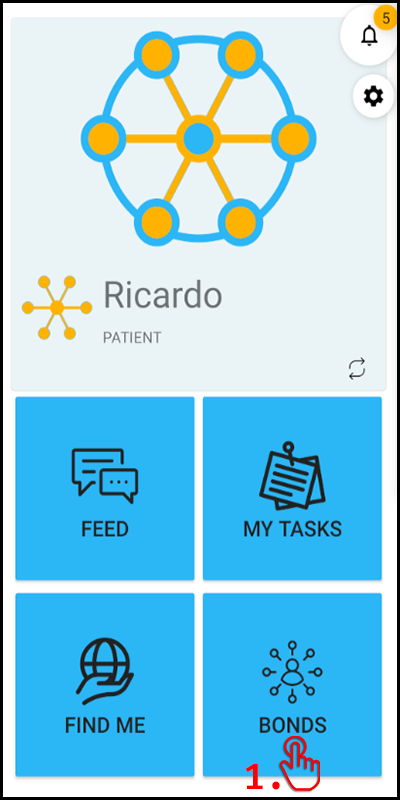
\includegraphics[width=.8\textwidth]{Manuales/ManualAccesoBonds.png}
    \end{minipage}\hfill
    \begin{minipage}{0.30\textwidth}
        \centering
        \includegraphics[width=.8\textwidth]{Manuales/ManualAñadirVinculo.png}
    \end{minipage}\hfill
    \begin{minipage}{0.30\textwidth}
        \centering
        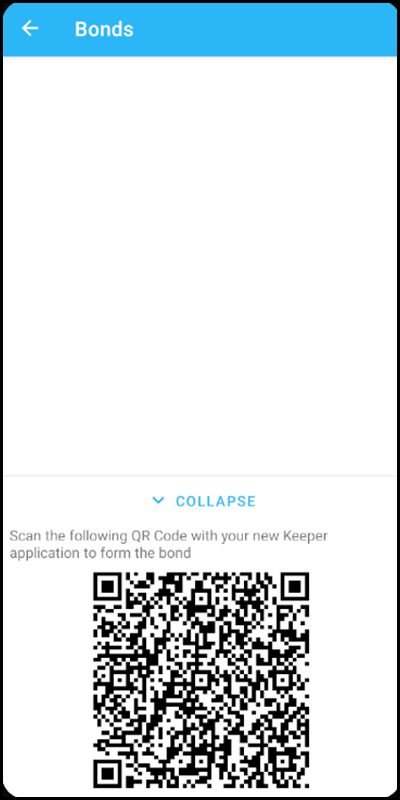
\includegraphics[width=.8\textwidth]{Diseño/CapturaBoundB.png}
    \end{minipage}\hfill
    \caption{Guía de generación de código QR de vinculación}
    \label{man:generar_qr}
\end{figure}

\subsection{Cuidador - Escanear código de vinculación}

\begin{figure}[H]
    \centering
    \begin{minipage}{0.5\textwidth}
        \centering
        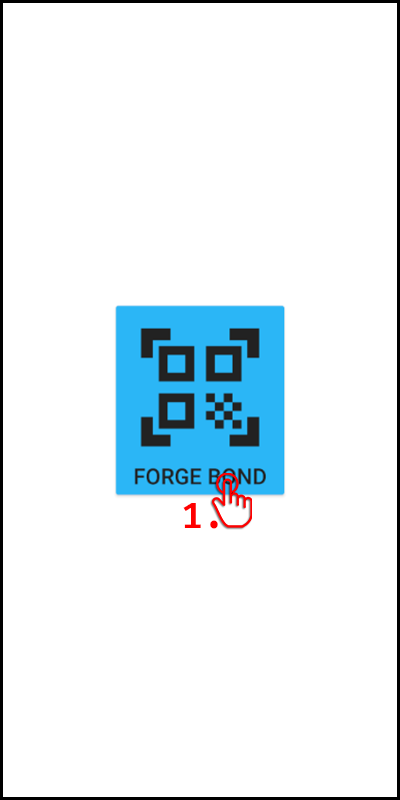
\includegraphics[width=0.5\textwidth]{Manuales/ManualAccesoEscaner.png}
    \end{minipage}\hfill
    \begin{minipage}{0.5\textwidth}
        \centering
        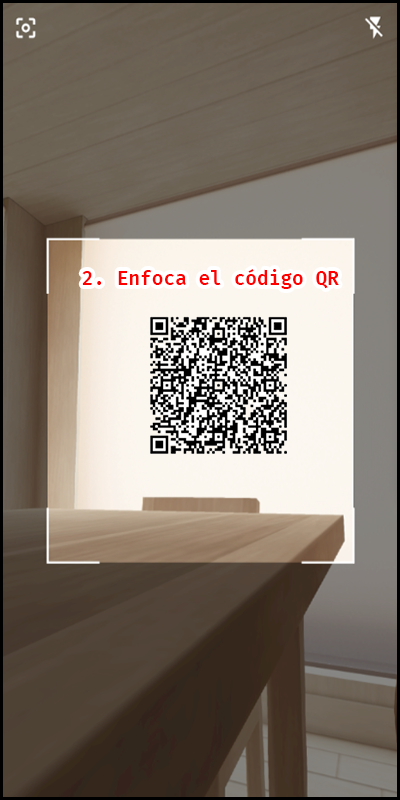
\includegraphics[width=0.5\textwidth]{Manuales/ManualEscaner.png}
    \end{minipage}\hfill
    \caption{Guía de escaneo del código QR de vinculación}
    \label{man:escanear_qr}
\end{figure}

Cuando te registras como cuidador sólo ves la pantalla que se muestra en la primera parte de \fref{man:escanear_qr}. Ese único botón despliega la \textbf{cámara} con un escáner para enfocar el código QR de la aplicación del paciente. Primero se te pedirá permiso para usar la cámara, si no lo concedes no será posible establecer el vínculo de otra manera. El centro de la cámara (la parte no oscurecida) indica donde deberías centrar el código para facilitar la lectura. Una vez que lo consigas escanear, \textbf{el vínculo se creará} y el Cuidador será dirigido a una pantalla principal similar a la de los pacientes con una tarjeta con los datos del Paciente.

\subsection{Consultar vínculos}

Si eres un usuario ya vinculado puedes consultar tus vínculos en la pantalla de \textbf{Vínculos} a la que se accede desde la pantalla principal como se indica en \fref{man:consultar_vinculos}. En esta página aparecerá una tarjeta por cada vínculo directo si eres un Paciente o por cada vínculo de tu Paciente si eres un cuidador. Cada una de estas tarjetas lleva el nombre de uno de estos y usando la flecha de la misma se puede desplegar el resto de la información del usuario.

\begin{figure}[H]
    \centering
    \begin{minipage}{0.5\textwidth}
        \centering
        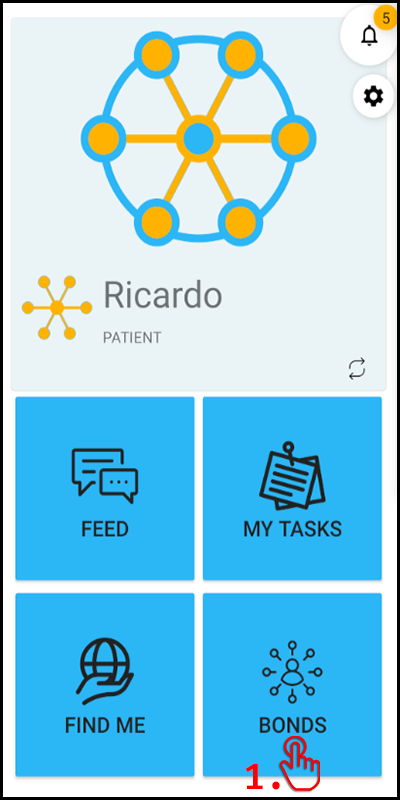
\includegraphics[width=0.5\textwidth]{Manuales/ManualAccesoBonds.png}
    \end{minipage}\hfill
    \begin{minipage}{0.5\textwidth}
        \centering
        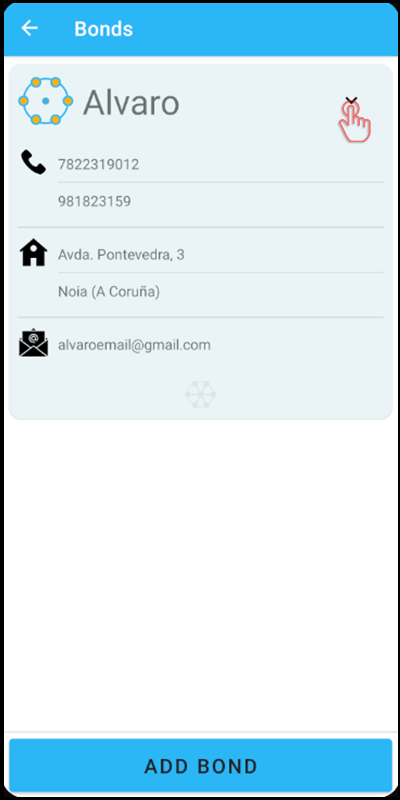
\includegraphics[width=0.5\textwidth]{Manuales/ManualListaVinculos.png}
    \end{minipage}\hfill
    \caption{Guía de consulta de vínculos}
    \label{man:consultar_vinculos}
\end{figure}

\subsection{Eliminar vínculos}

Los vínculos de los usuarios se eliminan desde lugares diferentes (mostrados en \fref{man:eliminar_vinculos}) seas un Paciente o un Cuidador. Los Pacientes podéis eliminar los vínculos desde la pantalla de \textbf{Vínculos} manteniendo pulsado sobre el vínculo que se quiera eliminar. Los Cuidadores en cambio lo podéis hacer desde \textbf{Ajustes}, con la opción \textbf{Eliminar vínculo}. En ambos casos se pedirá confirmación antes de llevarlo a cabo.

\begin{figure}[H]
    \centering
    \begin{minipage}{0.30\textwidth}
        \centering
        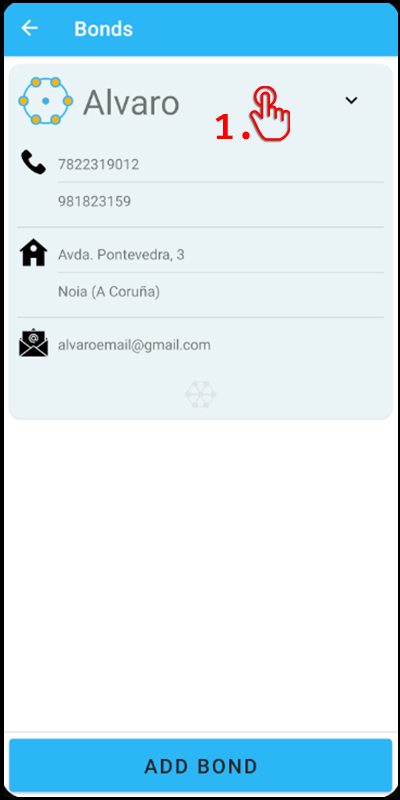
\includegraphics[width=.8\textwidth]{Manuales/ManualEliminarVinculoPaciente.png}
    \end{minipage}\hfill
    \begin{minipage}{0.30\textwidth}
        \centering
        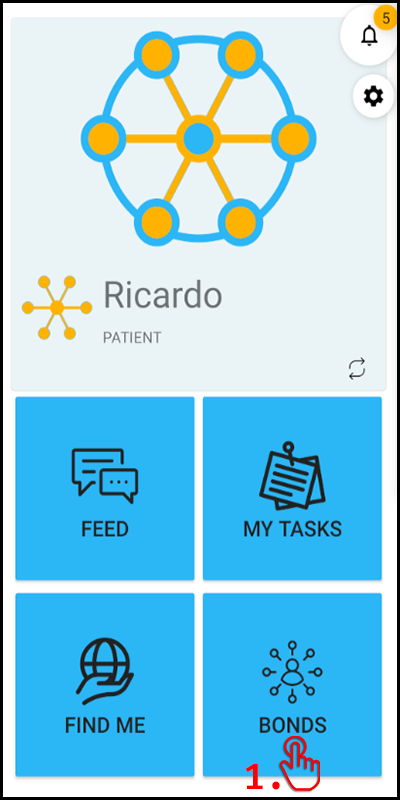
\includegraphics[width=.8\textwidth]{Manuales/ManualAccesoBonds.png}
    \end{minipage}\hfill
    \begin{minipage}{0.30\textwidth}
        \centering
        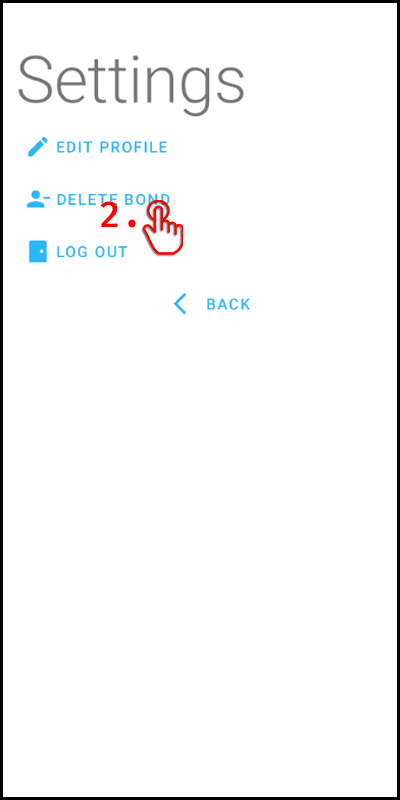
\includegraphics[width=.8\textwidth]{Manuales/ManualEliminarVinculoCuidador.png}
    \end{minipage}\hfill
    \caption{Guía de eliminación de vínculos}
    \label{man:eliminar_vinculos}
\end{figure}

\section{Geolocalización}

La geolocalización se encuentra disponible en la pantalla principal con el botón con el icono del globo como se indica en \fref{man:geolocalizacion}. Esto despliega un mapa a pantalla completa que se maneja de forma similar a cualquier otro mapa basado en \textbf{Google Maps}. Se te solicitará acceder al permiso a tu ubicación, si quieres compartirla con tus usuarios vinculados, concédela. 

\begin{figure}[H]
    \centering
    \begin{minipage}{0.5\textwidth}
        \centering
        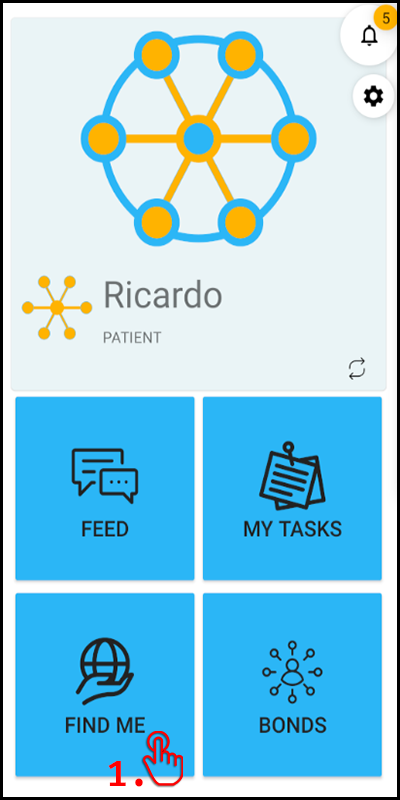
\includegraphics[width=0.5\textwidth]{Manuales/ManualAccesoMapa.png}
    \end{minipage}\hfill
    \begin{minipage}{0.5\textwidth}
        \centering
        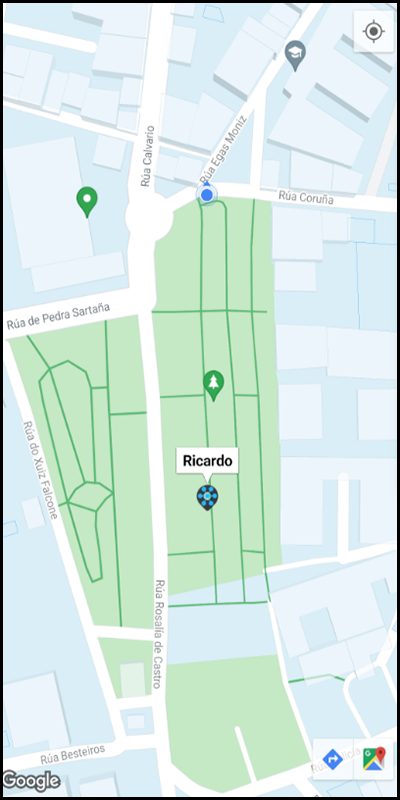
\includegraphics[width=0.5\textwidth]{Diseño/CapturaLocalización.png}
    \end{minipage}\hfill
    \caption{Guía de uso de geolocalización}
    \label{man:geolocalizacion}
\end{figure}

Cuando accedes a la página de geolocalización y comienzas a compartir tu ubicación, \textbf{una notificación será enviada} al resto de usuarios. De esta forma, si un Paciente comienza a compartir su ubicación todos sus Cuidadores lo sabrán, y si un Cuidador lo hace tanto Pacientes como Cuidadores vinculados también serán avisados de que este ha comenzado una búsqueda.

El manejo del mapa sigue los controles habituales. El mapa se puede mover deslizándose, se puede hacer \emph{zoom in} y \emph{zoom out} con el gesto de juntar o separar los dedos respectivamente. El botón de la esquina superior derecha centra el mapa en la posición del usuario, al usarlo el mapa seguirá al usuario cuando se actualice su ubicación salvo que lo desplace manualmente.

Por último, siempre que otro usuario acceda a esta misma pantalla y empiece a compartir su ubicación \textbf{se mostrará un marcador} de un color único representando a dicho usuario. Pulsando en los marcadores de los usuarios se \textbf{mostrará el nombre} del usuario al que pertenece.

\section{Enviar mensajes}
\label{sec:manual_enviar_mensajes}

La función de enviar mensajes está en el \textbf{Feed}. Su uso es igual que el de cualquier otro chat. Pulsando el campo de texto de la parte inferior se desplegará el teclado y se podrá escribir el mensaje que se desee enviar. El botón azul a la derecha de dicho campo sirve para enviarlo.

Esta sala de chat estará integrada por el Paciente y por todos sus Cuidadores. Los mensajes se envían en tiempo real, pero también se podrán ver todos los mensajes que se hayan enviado mientras no se está conectado. Subiendo hacia arriba se puede acceder a mensajes más antiguos y al llegar al límite de los cargados se cargarán los siguientes hasta que no haya ninguno más.

\begin{figure}[h]
    \centering
    \begin{minipage}{0.5\textwidth}
        \centering
        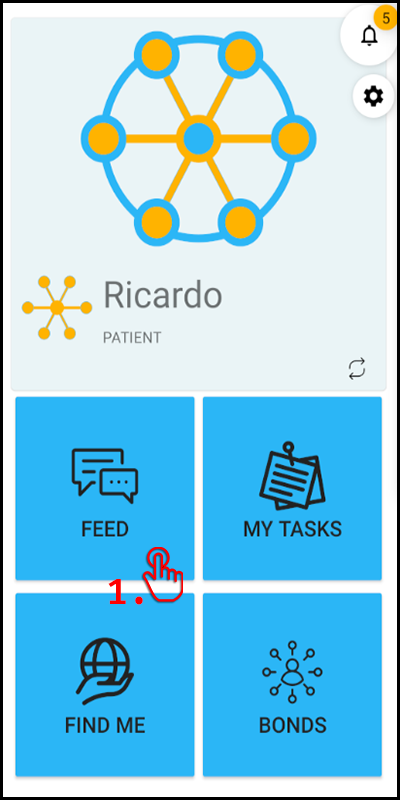
\includegraphics[width=0.5\textwidth]{Manuales/ManualAccesoFeed.png}
    \end{minipage}\hfill
    \begin{minipage}{0.5\textwidth}
        \centering
        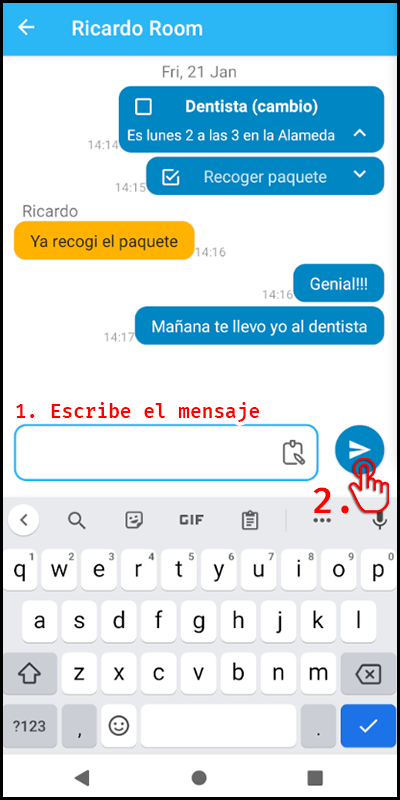
\includegraphics[width=0.5\textwidth]{Manuales/ManualEnviarMensaje.png}
    \end{minipage}\hfill
    \caption{Guía de envío de mensajes}
    \label{man:enviar_mensaje}
\end{figure}

\section{Gestionar tareas}

\begin{figure}[H]
    \centering
    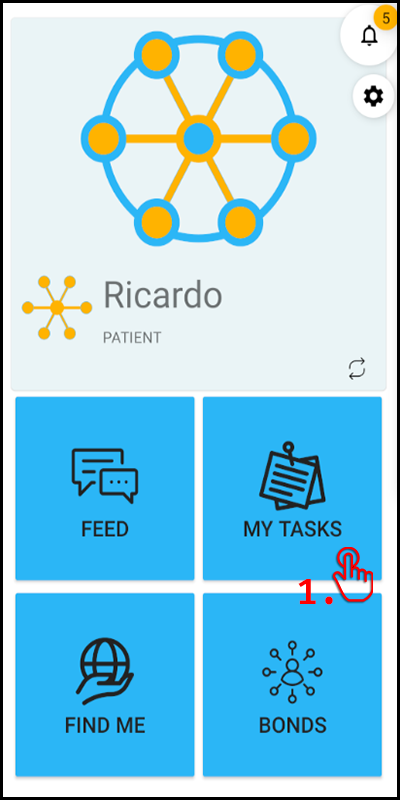
\includegraphics[width=0.25\textwidth]{Manuales/ManualAccesoTareas.png}
    \caption{Guía de acceso a Tareas}
    \label{man:tareas}
\end{figure}

Las tareas se pueden crear, marcar o desmarcar como hechas y eliminar. Todas estas acciones se pueden llevar a cabo desde la pantalla de \textbf{Tareas} (\fref{man:tareas}) y desde la pantalla de \textbf{Feed} (véase \fref{sec:manual_enviar_mensajes}).

\subsection{Crear tarea}

Para crear una tarea desde \textbf{Tareas} se debe pulsar el botón flotante de la esquina inferior derecha con el icono del portapapeles (véase \fref{man:crear_tarea}). Esto desplegará una ventana con el título de \textbf{Crear tarea} y dos campos de texto. Introduce el \textbf{título} de la tarea en el primero, el título será la información más básica de la tarea, procura que sea representativo y conciso. 

El otro campo de texto, de mayor tamaño, es para la \textbf{descripción}. La descripción es opcional, pero sirve de mucha utilidad para añadir detalles importantes de la tarea, de forma que el Paciente o los Cuidadores que la vayan a llevar a cabo tengan todas las facilidades posibles para hacerlo. Aprovecha este campo para introducir localizaciones, horas o nombres.

Una vez estés conforme con lo que has introducido, pulsa en \textbf{Crear} para finalizar la creación de la tarea y volver a la pantalla de Tareas donde la nueva tarea aparecerá listada. También puedes usar \textbf{Cancelar} si te arrepentiste y no quieres crear una tarea.

\begin{figure}[H]
    \centering
    \begin{minipage}{0.5\textwidth}
        \centering
        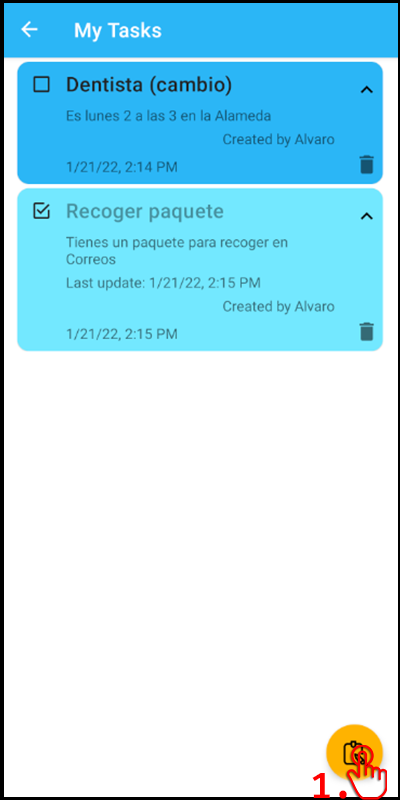
\includegraphics[width=0.5\textwidth]{Manuales/ManualAccesoCrearTarea.png}
    \end{minipage}\hfill
    \begin{minipage}{0.5\textwidth}
        \centering
        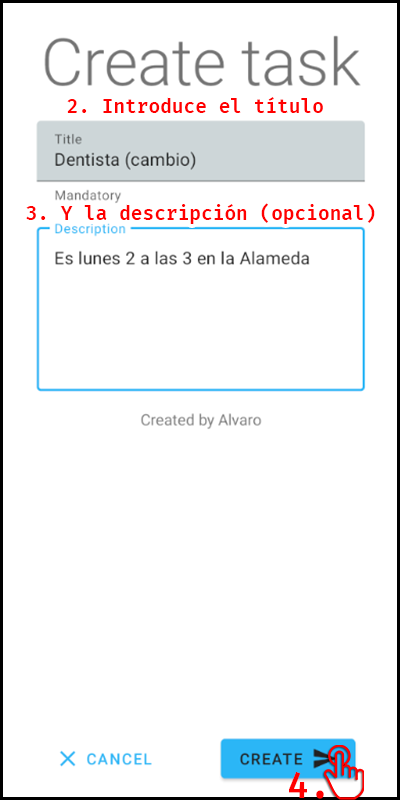
\includegraphics[width=0.5\textwidth]{Manuales/ManualCrearTarea.png}
    \end{minipage}\hfill
    \caption{Guía de creación de tareas a través de Tareas}
    \label{man:crear_tarea}
\end{figure}

El otro sistema para crear una tarea es a través del \textbf{Feed}. En el mismo encontrarás un icono de portapapeles dentro del campo de texto, pulsarlo desplegará el \textbf{modo tarea} (\fref{man:enviar_tarea}). En este modo aparecerá un área de texto adicional. Ahora el campo de texto de enviar mensajes sirve para introducir el \textbf{título} y la nueva área para la \textbf{descripción}. Sigue las mismas indicaciones que antes y cuando estés conforme envía la tarea con el mismo botón de \textbf{enviar mensajes}. La tarea aparecerá en tu chat y el de tus usuarios asociados. Si, en cambio, quieres salir del modo tarea puedes usar la equis que sustituyó al icono del portapapeles.

\begin{figure}[H]
    \centering
    \begin{minipage}{0.5\textwidth}
        \centering
        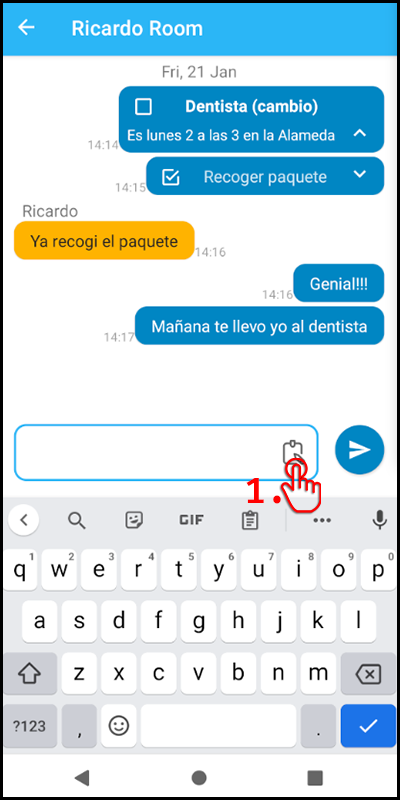
\includegraphics[width=0.5\textwidth]{Manuales/ManualModoTarea.png}
    \end{minipage}\hfill
    \begin{minipage}{0.5\textwidth}
        \centering
        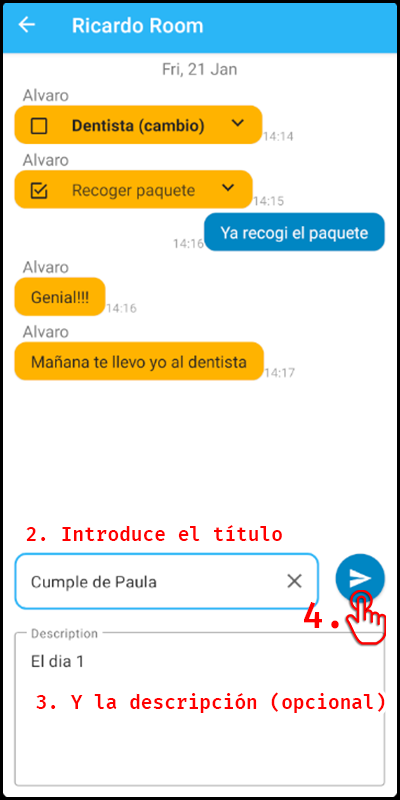
\includegraphics[width=0.5\textwidth]{Manuales/ManualEnviarTarea.png}
    \end{minipage}\hfill
    \caption{Guía de creación de tareas a través de Feed}
    \label{man:enviar_tarea}
\end{figure}

\subsection{Marcar y desmarcar tareas}

Tanto desde \textbf{Tareas} como desde el \textbf{Feed} se pueden modificar las tareas de la misma forma. Para lo primero se debe pulsar en la casilla de \emph{check} de la tarea. Si está vacía la tarea no está hecha y pulsarla la marcará como hecha y lo notificará a los usuarios interesados. Si por el contrario la casilla tiene un \emph{tick} (y se ve de un color más pálido) entonces estará marcada como hecha, pulsar la casilla en este caso logrará el efecto contrario, marcará la tarea como no hecha. Esto es útil si se marca por error o si una tarea que se creía hecha en realidad no lo estaba.

\subsection{Eliminar tareas}

La eliminación de tareas es distinta si se lleva a cabo desde el \textbf{Feed} y desde \textbf{Tareas}. En Tareas podrás encontrar un \textbf{icono  de papelera}, al pulsar se te preguntará si la quieres eliminar, una vez confirmes se borrará de tu lista de tareas y de todas. Para eliminar una tarea en el feed debes localizarla y \textbf{mantener pulsado encima}. La larga pulsación desplegará el mismo diálogo de confirmación y aceptarlo eliminará la tarea. Sin embargo, esta acción comparte el mismo requisito en ambos lados, sólo puedes eliminar una tarea si eres \textbf{el Paciente} o si eres \textbf{el creador} de la misma

\begin{figure}[H]
    \centering
    \begin{minipage}{0.5\textwidth}
        \centering
        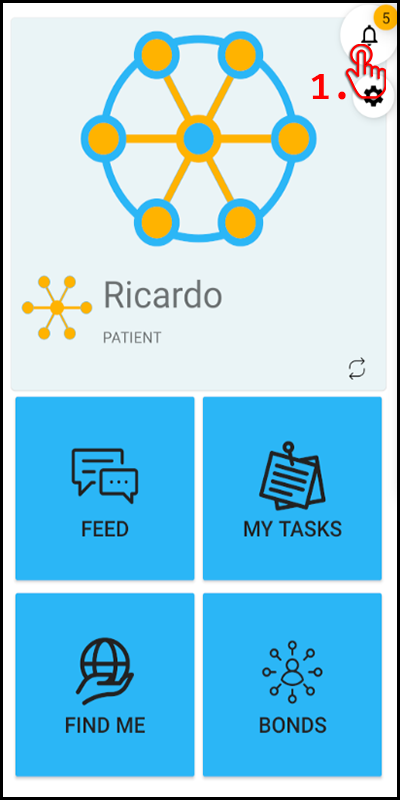
\includegraphics[width=0.5\textwidth]{Manuales/ManualAccesoNotificaciones.png}
    \end{minipage}\hfill
    \begin{minipage}{0.5\textwidth}
        \centering
        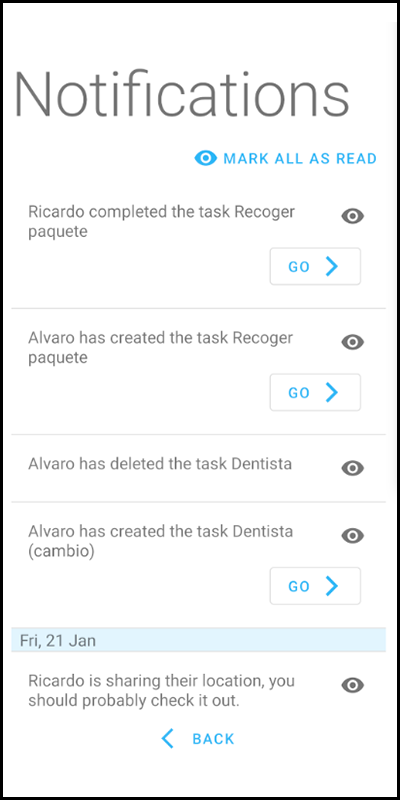
\includegraphics[width=0.5\textwidth]{Diseño/CapturaNotificaciones.png}
    \end{minipage}\hfill
    \caption{Guía de consulta de notificaciones}
    \label{man:notificaciones}
\end{figure}

\section{Consultar notificaciones}

En la parte superior de la pantalla principal hay un icono con forma de \textbf{campana}. En ocasiones este icono puede tener un número encima, si es el caso, este número indica la cantidad de notificaciones pendientes del usuario. Pulsar en dicho botón flotante (\fref{man:notificaciones}) desplegará una pantalla con la lista de notificaciones aún no leídas. 

Algunas de estas notificaciones tendrán un botón \textbf{Ir}. Estas notificaciones están relacionadas con otras pantallas y con dicho botón podrás acceder rápidamente al destino deseado. Por ejemplo, cuando un usuario vinculado empieza a compartir su ubicación recibirás una notificación indicándotelo y el botón \emph{Ir} de la misma te llevará directamente a la pantalla del mapa.

Las notificaciones pueden marcarse como leídas haciendo uso del icono con forma de \textbf{ojo} de su derecha. Al hacerlo esa notificación desaparecerá para siempre. También puedes agilizar esto usando la función \textbf{Marcar todas como leídas} de la parte superior. Esto señalará todas las notificaciones actuales como leídas y vaciará la pantalla completa.

\vspace{-15pt}
\section{Editar datos}

Desde \textbf{Ajustes}, pantalla a la que se accede desde el botón con forma de \textbf{engranaje} de la pantalla principal, puedes actualizar tus datos de usuario. Para ello debes seguir los pasos de la \fref{man:editar_perfil}. Primero despliega los campos de edición pulsando en \textbf{Editar perfil}. Una vez se desplieguen, modifica aquellos campos que quieras cambiar. Cuando estés satisfecho con los datos, completa la acción pulsando en \textbf{Confirmar}. En cualquier momento puedes usar \textbf{Cancelar} para cerrar los campos y abortar la operación.

\vspace{-15pt}
\begin{figure}[H]
    \centering
    \begin{minipage}{0.5\textwidth}
        \centering
        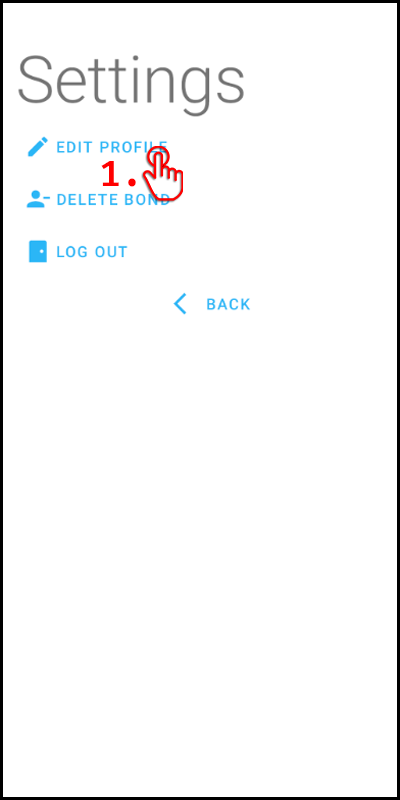
\includegraphics[width=0.5\textwidth]{Manuales/ManualAccesoEditarPerfil.png}
    \end{minipage}\hfill
    \begin{minipage}{0.5\textwidth}
        \centering
        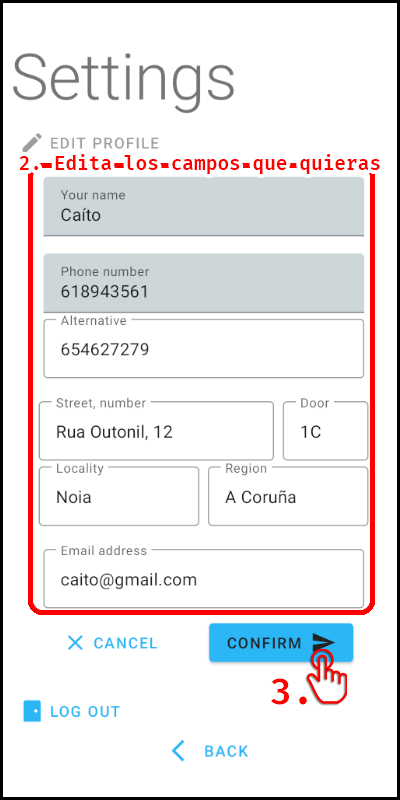
\includegraphics[width=0.5\textwidth]{Manuales/ManualEditarUsuario.png}
    \end{minipage}\hfill
    \caption{Guía de edición del perfil}
    \label{man:editar_perfil}
\end{figure}